\documentclass[10pt]{beamer}
\usetheme{metropolis}


\usepackage{appendixnumberbeamer}
\usepackage{booktabs}
\usepackage[utf8]{inputenc}
\usepackage[scale=2]{ccicons}
\usepackage{graphicx}
\usepackage{pgfplots}
\usepgfplotslibrary{dateplot}

\usepackage{xspace}
\newcommand{\themename}{\textbf{\textsc{metropolis}}\xspace}

\title{Ethik}
\subtitle{in Forschung und Gesellschaft}
\date{\today}
\author{Luca Lach und Sebastian Mueller}
\institute{}

\begin{document}
		
	\maketitle
	
	\begin{frame}{Inhaltsverzeichnis}
		\setbeamertemplate{section in toc}[sections numbered]
		\tableofcontents[hideallsubsections]
	\end{frame}
	
\section{Definition Ethik}
	\begin{frame}{Grundbegriff: Ethik}
		\textbf{Was ist Ethik?}
	\end{frame}
	
	\begin{frame}{Ethik vs. Moral}
		\textbf{Moral}
			\begin{itemize}
				\item Regeln der Gesellschaft für sozial verträgliches Verhalten
				\item verändert sich je nach aktuellen Gesellschaftsnormen
			\end{itemize}
		\textbf{Ethik}
		\begin{itemize}
			\item Regeln der Gesellschaft für sozial verträgliches Verhalten
			\item verändert sich je nach aktuellen Gesellschaftsnormen
		\end{itemize}
			
	\end{frame}
		

	
\subsection{Entwicklung des Ethikbegriffs}
	\begin{frame}{Ethikbegriff in der Geschichte}
		\textbf{Aristoteles} (384 v. Chr. - 322 v. Chr)
		\begin{itemize}
			\item tugendhaftes, gemeinnützuges Verhalten
		\end{itemize}
		
		\textbf{Pierre Abaillard} (1079 - 1142)
		\begin{itemize}
			\item Handlungen ethisch, wenn sie Gottes Willen ensprachen
		\end{itemize}
		
		\textbf{Jeremy Bentham und John Stuart Mill} (17. Jahrhundert)
		\begin{itemize}
			\item "Handle und entscheide Dich stets so, dass das Glück der
			meisten Menschen gefördert wird"
		\end{itemize}
	\end{frame}
	
	\begin{frame}{Ethikbegriff in der Geschichte}
		\textbf{Immanuel Kant} (1724 -1804)
		\begin{itemize}
			\item kategorischer Imperativ
		\end{itemize}
		
		\textbf{John Rawls} (1921 – 2002) 
		\begin{itemize}
			\item Jeder hat Anspruch auf Grundfreiheiten
			\item Soziale und ökonomische Ungleichheiten stark reguliert
		\end{itemize}
	\end{frame}
	%Moralphilosophie, Entstehung des Begriffs, Disziplinen, worauf wir uns konzentrieren werden
	%Wandelnde Weltanschauungen -> Wandelndes Verstaendnis der Ethik
	%Mittelalter: goettliche ordnung -> religioese Ethik
	%Neuzeit: Utilitarismus, Egoistische Ethik, 
	%Verankerung ethischer Normen in der modernen Gesellschaft -> Grundgesetz, Richtlinien, im Vortrag nun also insbesondere Richtlinien in der Forschung 
	%-> Rechte auf Selbstbestimmung, Gesundheit, persoenliche Entfaltung
\section{Ethische Richtlinien in der experimentellen Forschung}
	\begin{frame}{Relevanz der Ethik in der experimentellen Forschung}
		Perspektive der Versuchsperson:
		\begin{itemize}
		%	\item Unversehrtheit der Versuchsperson steht im Vordergrund
			%\item Forschung angewiesen auf Versuchspersonen
		%	\item Versuchsleiter 
		\item Möchte mitwirken an Forschung	%hilft freiwillig,
		\item Begibt sich in unbekannte Situation
		\item Gibt Kontrolle an Versuchsleiter ab %vertraut dem Versuchsleiter 
		\end{itemize}
		
	\end{frame}
	
	
		\begin{frame}{Little-Albert Experiment [1920]}
			Ziel: Anzahl von Reizen die eine emotionale Reaktion auslösen kann mit einfachen Mitteln vermehrt werden\\
			
			Ablauf:
			\begin{itemize}
				\item Erster Durchlauf: Man zeigte Albert ihm unbekannte Lebewesen und Gegenstände
				\item Zweiter Durchlauf: Erneutes zeigen von den Lebewesen und Gegenstaenden begleitet von lautem Geräusch
				\item Dritter Durchlauf: Ähnliche Reize provozieren emotionale Reaktion
			\end{itemize}
					\end{frame}
	
	\begin{frame}{Little-Albert Experiment [1920]}
		
		\begin{itemize}
			\item Forscher haben mit bleibenden psychischen Schäden bei Albert gerechnet
			\item Mutter fühlte sich zur Teilnahme gedrängt
			\item Albert nicht mündig
		\end{itemize}
		$\Rightarrow$ \textbf{unfreiwillige} Teilnahme, bleibende \textbf{psychische Schäden} der VP
	\end{frame}

	
	\begin{frame}{Richtlinien}
		
		\begin{itemize}
			\item Arbeite mit freiwilligen VP zusammen
			\item Nutze VP nicht aus
			\item Schließe negative Folgen für die Teilnehmer aus
		\end{itemize}
		
	\end{frame}
	
	\begin{frame}{Robber's Cave [1954]}
		Ziel: Erforschung der Entstehung und Schlichtung von Gruppenkonflikten\\
		Ablauf:
		\begin{itemize}
			\item VPs wurden zufällig in zwei gleichgroße Gruppen aufgeteilt
			\item Gruppen führten getrennt voneinander Aktivitäten durch
			\item Provokation von Konflikten durch die unfaire Beeinflussung eines Wettkampfs zwischen den Gruppen
			\item Versuchte Schlichtung der Konflikte durch Kooperation der beiden Gruppen zum erreichen gemeinsamer Ziele
		\end{itemize}
		
	\end{frame}	

	\begin{frame}{Robber's Cave [1954]}
		Ziel: Erforschung der Entstehung und Schlichtung von Gruppenkonflikten\\
		Ablauf:
		\begin{itemize}
			\item Die Gruppen wussten nicht um Manipulation des Wettkampfs
			\item Teilnehmer wurden nicht über Ziele der Studie aufgeklärt
		\end{itemize}
		$\Rightarrow$ bewusste \textbf{Täuschung} der Teilnehmer
	\end{frame}	

	\begin{frame}{Richtlinien}
		
		\begin{itemize}
			\item Arbeite mit freiwilligen VP zusammen
			\item Nutze VP nicht aus
			\item Schließe negative Folgen für die Teilnehmer aus
			\item Sei offen und ehrlich
			\item Informiere Teilnehmer und schliesse mit ihm eine Übereinkunft
			\item Kläre adäquat auf
		
		\end{itemize}
		
	\end{frame}
	
	\begin{frame}{Stanford Prison [1971]}
		Ziel: Wie schnell adaptieren VP erwartete Verhaltensweisen ihrer Rollen \\
		
		Ablauf:
		\begin{itemize}
			\item VPs eingeteilt in Wärter und Gefangene
			\item Gefangene traten von Grundrechten ab und wurden öffentlich verhaftet
			\item VPs simulierten Gefängnisalltag in zugeteilten Rollen
			\item Wärter hatten volle Handlungsfreiheit gegenüber der Gefangenen
		\end{itemize}
		
	\end{frame}	
	
	\begin{frame}{Stanford Prison [1971]}
		\begin{itemize}
			\item Abbruchmöglichkeiten seitens der Teilnehmer nicht klar
			\item VL ließen Schädigung und Diskirminierung der Gefangenen bewusst zu
			\item negative soziale Konsequenzen durch Festnahme
		\end{itemize}
		$\Rightarrow$ \textbf{physischer Schaden} der Teilnehmer \& \textbf{öffentliche} Demütigung
	\end{frame}	
	
	\begin{frame}{Richtlinien}
		
		\begin{itemize}
			\item Arbeite mit freiwilligen VP zusammen
			\item Nutze VP nicht aus
			\item Schließe negative Folgen für die Teilnehmer aus
			\item Sei offen und ehrlich
			\item Informiere Teilnehmer und schliesse mit ihm eine Übereinkunft
			\item Kläre adäquat auf
			\item Schütze Teilnehmer vor Schaden
			\item Wäge Kosten \& Nutzen ab
			\item Übernimm Verantwortung
			\item Bewahre Vertraulichkeit
		\end{itemize}
		
	\end{frame}
	
	\begin{frame}{Das Milgram Experiment [1961]}
		
		%	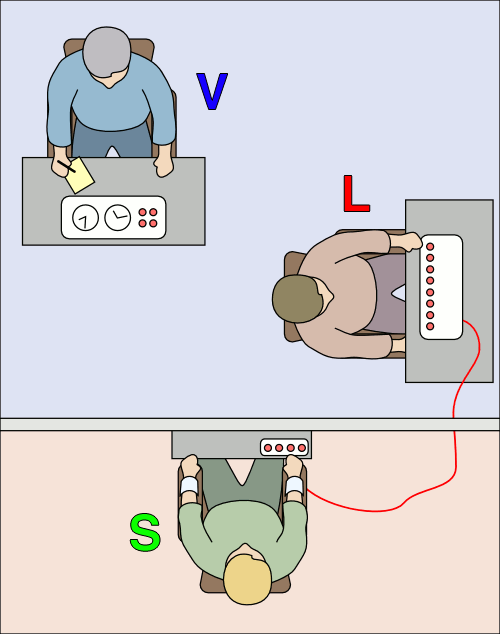
\includegraphics[scale=0.25]{./pics/Milgram_Experiment.png}
		Ziel: Grad der Gehorsamkeit gegenüber einer Autoritätsperson in moralischer Konfliktsituation messen\\
		
		Ablauf:
		\begin{itemize}
			\item VP ist "Lehrer"
			\item Überprüft Gedächtnisleistung einer anderen Person
			\item Bei Fehler soll VP Elektroschock auslösen
			\item Weigert sich VP weitere Elektroschocks zu erteilen befiehlt der VL das Weitermachen
		\end{itemize}
		
	\end{frame}
	
	\begin{frame}{Das Milgram Experiment [1961]}
		Was hat Milgram falsch gemacht?
			\begin{itemize}
				\item Arbeite mit freiwilligen VP zusammen
				\item Nutze VP nicht aus
				\item Schließe negative Folgen für die Teilnehmer aus
				\item Sei offen und ehrlich
				\item Informiere Teilnehmer und schliesse mit ihm eine Übereinkunft
				\item Kläre adäquat auf
				\item Schütze Teilnehmer vor Schaden
				\item Wäge Kosten \& Nutzen ab
				\item Übernimm Verantwortung
				\item Bewahre Vertraulichkeit
			\end{itemize}
	\end{frame}

\section{Ethisch diskutable Themen in der Informatik}
	

	
	\begin{frame}{Interaktives Roboterexperiment}
		\textbf{Ziel}: intuitives Verhalten mit Robotern erforschen\\
		\vspace{0.8cm}
		\textbf{Ablauf}:
		\begin{itemize}
			\item VP erhielt Richtungsanweisungen für gewünschte Bewegung des Roboters
			\item VL überwachte VP aus dem Nebenraum und kontrollierte den Roboter
			\item VL ließ Roboter nach Interaktion die geforderte Bewegung ausführen
		\end{itemize}
	\end{frame}
	
	\begin{frame}{Interaktives Roboterexperiment}

		\begin{itemize}
			\item VP wurden im Nachhinein über Täuschung aufgeklärt
			\item Person mit Notausschalter befand sich immer im Raum mit Roboter \& VP
		\end{itemize}
	\end{frame}
	
	\begin{frame}{VR: Agency detection in predictive minds}
		Ziel: Wie beeinflusst sensorische Beeinflussung bzw. daraus resultierender Stress das Wahrnehmen unbelebter Natur \\
		Ablauf:
		\begin{itemize}
		\item Teilnehmer macht zwei Spaziergaenge im Wald bei je unterschiedlichen Wetterbedingungen
		\item Bedingungen: Tag, Nebel, Nacht
		\item Teilnehmer wird gesagt das er wahrscheinlich Lebewesen begegnen wird und soll einen Knopf drücken wenn er meint das eins da ist
		\end{itemize}
	\end{frame}
	
	
	\begin{frame}{VR: Agency detection in predictive minds}
		
		\begin{itemize}
			\item Es gab keine Lebewesen im Wald
			\item Übelkeit und Schwindel sind bekannte Nebenwirkungen in VR-Simulationen
			\item Nachtsituation war zwischenzeitlich sehr gruselig
		\end{itemize}
		
	\end{frame}

	\begin{frame}{Prothetik}
	
	\end{frame}
		
		\begin{frame}{RoboCup}
			\begin{itemize}
				\item internationaler Wettkampf von Teams mit ihren Robotern
				\item entstand als Fußballwettkampf
				\item weitete sich immer mehr auf verschiedene Teilbereiche des Alltags aus
				\item Teilnahme an der @Home Liga
				\item Sicherheitsprüfung der einzelnen Roboter
				\item Roboter müssen Aufgaben in Haushaltsszenario erfüllen
				\item erreichen von Teilaufgaben wird bepunktet
				\item Präsentation frei erfundener Szenarien vor Laien 
			\end{itemize}
		\end{frame}
			\begin{frame}{RoboCup}
				\begin{itemize}
					\item KI findet immer mehr Verwendung im RoboCup
					\item Entscheidungen der Haushaltshelfer durch KI gefällt
					\item Sicherheitsmaßnahmen von Programmierer umgesetzt
				\end{itemize}
			\end{frame}
			\begin{frame}{Google}
				\textbf{SafeSearch}
				\begin{itemize}
					\item Bilder- und Textsuche zensiert anstößige Inhalte
					\item größtenteils gefiltert durch Algorithmen
					\item letzte Kontrolle durch Menschen
					\item ca 15.000 Bilder pro Tag mit extremen Inhalten
					\item wenig Nachsorge von Google aus gegenüber dem Mitarbeiter
				\end{itemize}
				\textbf{Suchalgorithmen}
				\begin{itemize}
					\item Nutzer werden unbewusst als VP benutzt
				\end{itemize}
			\end{frame}
	
	\begin{frame}{RoboCup}
		
	\end{frame}

	
\subsection{Motivation an kontroversem Experimenten}
%erste Diskussion was den Anwesenden auffaellt was da schief gelaufen sein koennte
% ein paar Konkrete Richtlinien ansprechen
\subsection{Richtlinien der APA}
%American Psychologie Association hat wegen diesen Kritiken folgende Richtlinien entwickelt
%
\subsection{Die Versuchsperson}
%freiwilliger Teilnehmer, moechte (idealerweise) der Forschung helfen
%Experiment
%Methodisch angelegte Untersuchung zur empirischen Gewinnung von Informationen. Ist eine kuenstliche Situation die vom Versuchsleiter geplant und herbeigefuehrtwird ueber die die VP dementsprechend nicht den vollen Ueberblick oder Kontrolle hat.
%daraus folgt besondere Verantwortung
\subsection{Wahrung der Selbstbestimmung}
%Aufklaerung, Vertrag schliessen
%Konflikt: Taeuschung von VP? Experiment Beispiel?

\subsection{Unwissende VP/ VP nicht ausnutzen}

\section{Design und Durchfuehrung ethisch korrekter Experimente}
%was der Text dazu sagt:
\subsection{Design}
%Grundsaeze: 1) Wahrung von Wuerde, Privatsphaere, psychische und physische Unversertheit; Ist die Gefaehrdung thematisch und/oder methodisch? Wie schwerwiegend wird die Beeintraechtigung eingeschaetzt? -> Voruntersuchung
%2) Herstellung von Transparenz; Teilnehmer vollstaendig ueber Untersuchungsgegenstand und Untersuchungsmaterialien informieren um ihnen eien informierte Entscheidung zu ermoeglichen ob sie bspw bei sensiblen Themen weiter Auskunft geben wollen
%3) Vermeidung von Taeuschungen;die Entscheidung muss man PERSOENLICH VERANTWORTEN KOENNEN WOW TOLL 
% Gespraeche mit anderen Wissenschaftlern [no shit shercock], alternative Untersuchungen planen (hierfuer vlt ein Beispiel durchsprechen? untersuchung die gegen ethische Richtlinien verstoesst so ummodellieren das sie ethisch in Ordnung ist)
\subsection{Durchfuehrung}
%Anwerben der VP -> keine zu grosse Belohnung anbieten?
%Aufklaerung -> offen und ehrlich sein, Vertrag schliessen! VP verpflichtet sich auch dazu die Untersuchung gewissenhaft zu absolvieren

\subsection{Beispiele aus den Fachbereichen Robotik, VR}
%Sensibilisierung in Fachbereich
% llachs BA
% semuellers Daene
% exposure therapy


\section{Diskussion: Ethik in der Informatik}
%Da Gesetze und Richtlinien nur die praktische Ausuebung unseres theoretischen Verstaendnisses von dem Ethikbegriff sind, sollten wir den Begriff nun auch in einem groesseren Kontext diskutieren um durch eine Einordnung in einen groesseren Kontext fuer das Thema zu sensibilisieren

%Zwangsrekrutierung Beispiel Google: Ist das ueberhaupt ein experiment? Warum fragen die nicht einfach ob man bei einem Beta-Test teilnehmen moechte?

%Verantwortung von uns als KI Forschern, wie gehen wir mit KI um?
%Arbeiten an moralisch fragwuerdigen Projekten oder erarbeiten von Wissen das bspw zur Kriegsfuehrung verwendet werden kann
% ai als produkt: Welche Verantwortung uebernehmen wir wenn wir Software vertreiben die komplexe/wichtige Aufgaben uebernimmt oder unterstuetzt deren Verhalten wir nicht in jeder Situation vorhersagen koennen. Wir programmieren ein komplexes Produkt das sich unvorhersehbar verhalten kann.
%Chirurgieroboter? Ueberwachungssoftware? Wie autonom darf diese Software sein? Wie sehr soll sich ein Mensch auf die Software verlassen duerfen? Was waeren ethisch korrekte Messgroessen um die beiden letzten Fragen beantworten zu koennen?

%Wie verhalten wir uns gegenueber KI?
% Minenroboter? Forscher hatten Mitleid beim Test von diesen Robotern; kann es zu einer schleichenden Verrohung kommen wenn wir humanoide Roboter ruecksichtslos "behandeln"?
%Selbstbewusste KI, welche Massstaebe wuerde man an die anlegen? Eigenen Willen respektieren? Man koennte sie einfach kopieren und mit der Kopie experimentieren und bei Schaeden danach loeschen?

\begin{frame}{Quellen}
	\begin{itemize}
		\item Ethik fuer Einsteiger von Dr Ulf D. Pose
		\item https://www.googlewatchblog.de/2012/08/googles-safesearch-filter-problemen/
		\item Agency detection in predictive minds: a virtual reality study von Marc Andersen et al.
	\end{itemize}
	
\end{frame}
\end{document}
